\begin{frame}{Pseudopotencial}
     \begin{columns}[t]
        \column{0.5\textwidth}
        \begin{figure}[H]
            \centering
            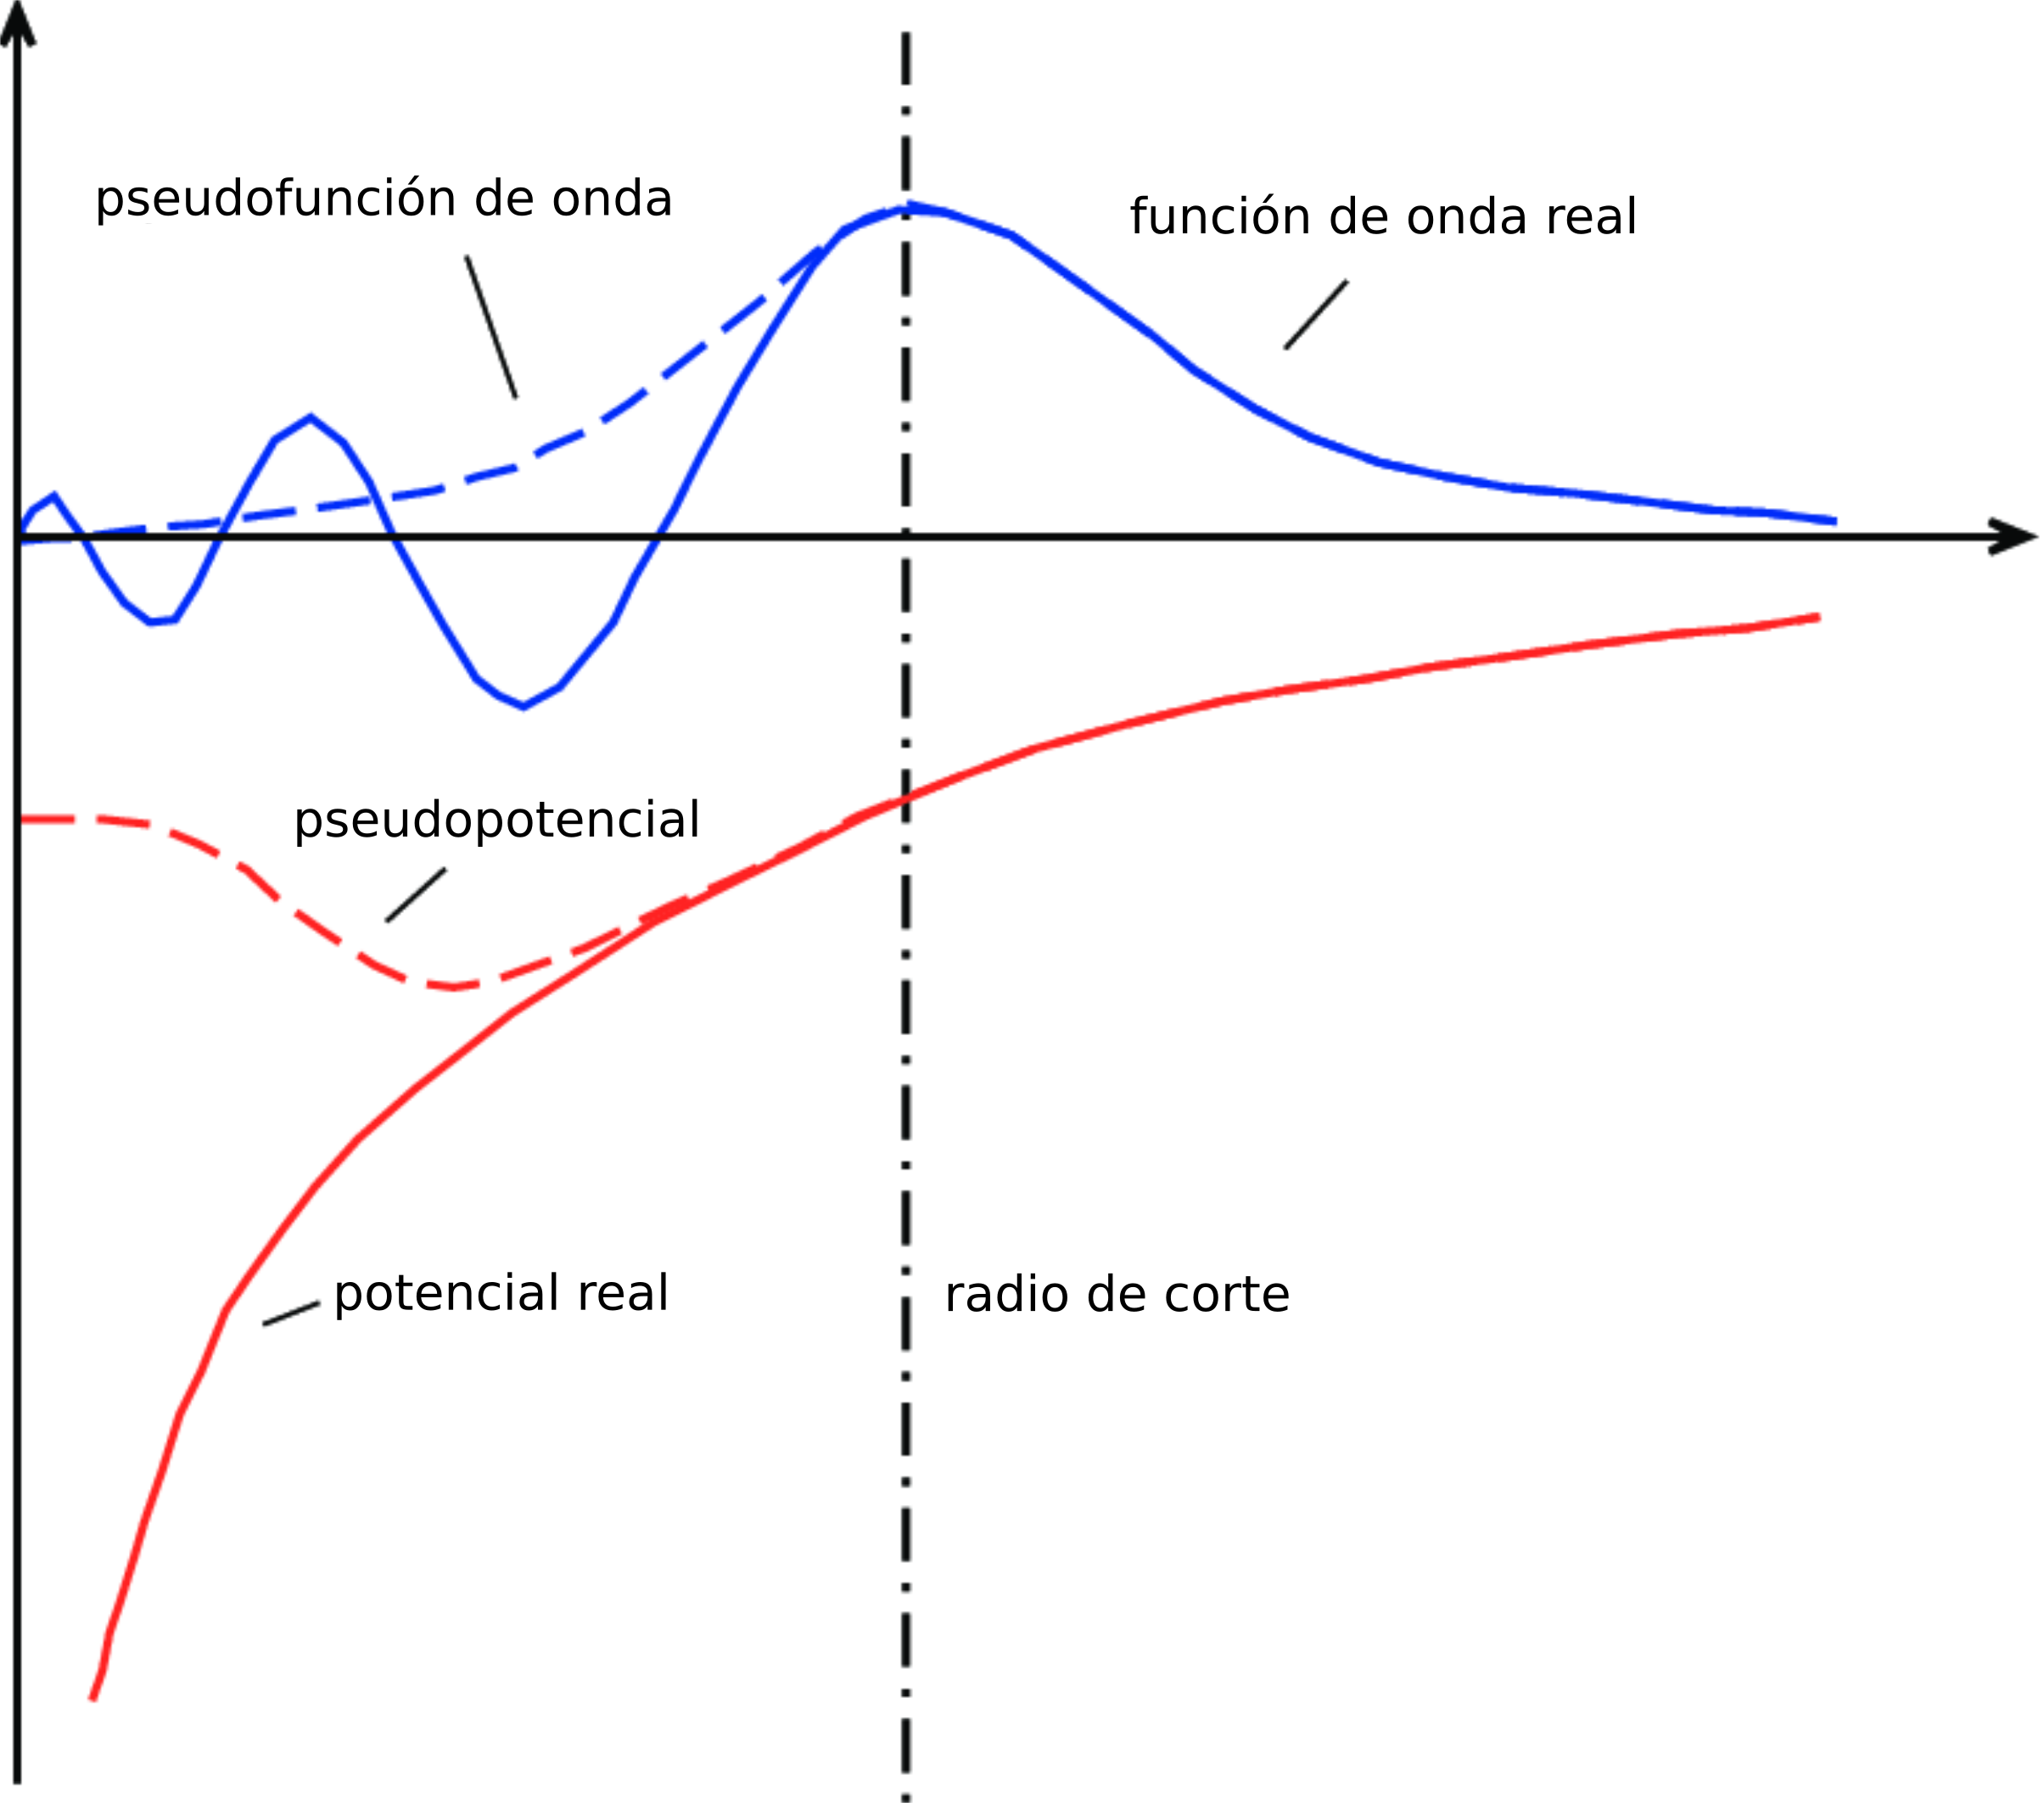
\includegraphics[width=1.0\textwidth]{contenido/teoria/img_teoria/pseudopotential.png}
            \caption{Representaci\'on del pseudopotencial}
        \end{figure}
        \column{0.5\textwidth}
        \begin{itemize}
            \item Reemplazo de las funciones de onda por pseudofunciones.
            \item Se define un radio de corte.
        \end{itemize}
    \end{columns}
    
\end{frame}